\documentclass[paper=a4, fontsize=12pt]{scrartcl} % A4 paper and 11pt font size

\usepackage[T1]{fontenc} % use 8-bit encoding that has 256 glyphs
\usepackage{fourier}     % use the Adobe Utopia font for the document
                         % (comment this line to return to the LaTeX default)
\usepackage[english]{babel} % English language/hyphenation
\usepackage{amsmath,amsfonts,amsthm} % math packages
\usepackage{subeqnarray}
\usepackage{manfnt}
\usepackage{lipsum} % used for inserting dummy 'Lorem ipsum' text into the template
\usepackage{bold-extra}
\usepackage{bclogo}
\usepackage{listings}
\usepackage[utf8]{inputenc}
\usepackage{amsthm}
\usepackage{amssymb}
% default fixed font does not support bold face
\DeclareFixedFont{\ttb}{T1}{txtt}{bx}{n}{11} % for bold
\DeclareFixedFont{\ttm}{T1}{txtt}{m}{n}{11}  % for normal

% custom colors
\usepackage{color}
\definecolor{deepblue}{rgb}{0,0,0.5}
\definecolor{deepred}{rgb}{0.6,0,0}
\definecolor{deepgreen}{rgb}{0,0.5,0}
\definecolor{lightblue}{rgb}{0.95,0.95,1}
\definecolor{lightgrey}{rgb}{0.6,0.6,0.6}
\usepackage{listings}

% use graphics packages
\usepackage{graphicx}
\usepackage{float}
\usepackage{tikz}
\usetikzlibrary{matrix}
\usetikzlibrary{calc}
\usetikzlibrary{patterns,fadings}

\graphicspath{ {images/} }
\newenvironment{claim}[1]{\par\noindent\underline{Claim:}\space#1}{}
\newenvironment{claimproof}[1]{\par\noindent\underline{Proof:}\space#1}{\hfill $\blacksquare$}
% python style for highlighting
\newcommand\pythonstyle{\lstset{
language=Python,
backgroundcolor=\color{lightblue},
basicstyle=\ttm,
    % add keywords here
keywordstyle=\ttb\color{deepblue},
emph={while,for,if,elif,else,def,as,shape,conj,dot,copy,flatten,eye,zeros,ones,hstack,vstack,real,imag,conjugate,sin,cos,exp,append,insert,index,__main__}, % custom highlighting
%emphstyle=\ttb\color{deepred},     % custom highlighting style
emphstyle=\ttb\color{deepblue},     % custom highlighting style
stringstyle=\color{deepgreen},
commentstyle=\color{lightgrey},
frame=tb,                         % any extra options here
numbers=left,
showstringspaces=false            %
}}

% python environment
\lstnewenvironment{python}[1][]
{
\pythonstyle
\lstset{#1}
}
{}

% python for external files
\newcommand\pythonexternal[2][]{{
\pythonstyle
\lstinputlisting[#1]{#2}}}

% python for inline
\newcommand\pythoninline[1]{{\pythonstyle\lstinline!#1!}}


\usepackage{sectsty}        % allows customizing section commands
\allsectionsfont{\centering \normalfont\scshape}      % make all sections centered
                                                      % the default font and small caps

\usepackage{fancyhdr}        % custom headers and footers
\pagestyle{fancyplain}       % makes all pages in the document conform to
                             % the custom headers and footers
\fancyhead{}                 % no page header - if you want one, create it in
                             % the same way as the footers below
\fancyfoot[L]{}              % empty left footer
\fancyfoot[C]{}              % empty center footer
\fancyfoot[R]{\thepage}      % page numbering for right footer
\renewcommand{\headrulewidth}{0pt}     % remove header underlines
\renewcommand{\footrulewidth}{0pt}     % remove footer underlines
\setlength{\headheight}{13.6pt}        % customize the height of the header

\numberwithin{equation}{section}       % number equations within sections
                                       % (i.e. 1.1, 1.2, 2.1, 2.2 instead of 1, 2, 3, 4)
\numberwithin{figure}{section}         % number figures within sections
                                       % (i.e. 1.1, 1.2, 2.1, 2.2 instead of 1, 2, 3, 4)
\numberwithin{table}{section}          % number tables within sections
                                       % (i.e. 1.1, 1.2, 2.1, 2.2 instead of 1, 2, 3, 4)

\setlength\parindent{0pt}         % removes all indentation from paragraphs
                                  % comment this line for an assignment with lots of text

%--------------------------
%	TITLE SECTION
%--------------------------

\newcommand{\horrule}[1]{\rule{\linewidth}{#1}} % create horizontal rule command
                                                % with 1 argument of height

\title{
\normalfont \normalsize
\textsc{Imperial College London, Department of Mathematics} \\ [25pt]
\horrule{0.5pt} \\[0.4cm]                      % thin top horizontal rule
\huge Scientific Computing (M3SC) Project 2 \\           % the assignment title
\horrule{2pt} \\[0.5cm]                        % thick bottom horizontal rule
}

\author{Omar Haque}
\date{\normalsize\today}

\begin{document}
%\ttfamily
%\fontseries{b}\selectfont

\maketitle

\section{Introduction}

In this coursework, I will use the algorithmic steps provided to design a workflow and job schedule that minimises the duration of the processes while maximising the number of processes that can be executed in parallel. \\
Rather than describing a strategy in one section and providing the implementation in another, I will be running through each of the sections and describing the code and theory simultaneously. 
\section{Extract data}
In order to make this program as robust and as general as possible, I have written a csv file which contains the data from Table 1.1 of the question, i.e the List of jobs, their duration and dependencies.
The function \textit{extract\_data} uses the csv module to iterate through every row of the datafile, and combine them into a numpy array.

\begin{python} 
import csv
import numpy as np
import sys


def extract_data(file_name):
    """
    This function uses the csv module to extract the 'jobs', 'durations'
    and 'has to be completed before' columns

    :param file_name: a csv file containing the data
    :return: a total_nodesx3 np.array containing the 'jobs', 'durations'
    and 'has to be completed before' columns
    """
    # e.g. file_name = './data/jobslist'
    job = []
    duration = []
    completed_before = []

    # open the file
    with open(file_name, 'r') as file:

        AAA = csv.reader(file)
        # iterate through each row
        for i, row in enumerate(AAA):
            # add the job number
            job.append(int(row[0]))
            # add the duration
            duration.append(int(row[1]))
            # if there are jobs to be completed before, add them
            if len(row) > 2:
                completed_before.append([int(node) for node in row[2:]])

            else:
                # else add an empty list. 
                completed_before.append([])

    file.close()

    # combine these together
    data_frame = np.column_stack((job, duration, completed_before))

    return data_frame
    \end{python}


Running this code then produces the array shown in figure \ref{data}
\begin{python}
data = extract_data('./data/jobslist')
\end{python}

\begin{figure}[t]
\caption{np.array produced from extract\_data}
\centering
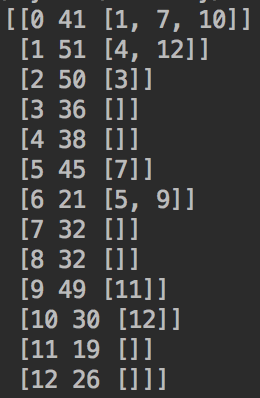
\includegraphics{data}\label{data}
\end{figure}

\section{Constructing the graph}
We now construct the directed graph, as described in steps \textbf{1,2,3} and \textbf{4} of algorithm 1.1 in the question. For job $m \in \{ 0,1,\dots, 12 \}$ I write $m_{s}$ and $m_{f}$ for the start and finish node for job m respectively. I also write $v_{s}$ and $v_{f}$ for the virtual start and virtual finish node respectively.

I will construct an adjacency matrix, $W = \{ w_{i,j} \}$, where $w_{i,j}$ denotes the edge weight between node $i$ and node $j$. The ordering of the matrix rows and columns is the following sequence $$ 0_{s} 1_{s} \dots 12_{s} 0_{f} 1_{f} \dots 12_{f} v_{s} v_{f}$$
The weights $w_{i,j}$ are specified by steps \textbf{1,2,3} and \textbf{4} of algorithm 1.1, I write the conditions here. $\forall$ jobs m,n $\in \{ 0,1,\dots 12\}$:
\begin{itemize}
  \item $w_{m_{s},m_{f}}$ = the duration of job m. By inspection, the duration of a job is always strictly positive.
  \item $w_{m_{f},n_{s}}$ = 0 if job m has to be completed before job n.
  \item $w_{v_{s},m_{s}} = 0$
  \item $w_{m_{f},v_{f}} = 0$
\end{itemize}

Else, we take a value of $w_{i,j} = -1$ if node $i$ is not connected to node $j$. 

Here is the python implementation:

\begin{python}
def generate_weight_matrix(data):
    """
    This function uses the data to create an adjacency matrix, based
    on the rules outlined.

    :param data: three column np.array with 'jobs', 'durations'
    and 'has to be completed before' columns
    :return: the adjacency matrix for this graph
    """
    global total_nodes, virtual_start, virtual_finish,job_duration
    # we start with an array of -1s and populate the entries that
    # correspond to connected nodes.
    total_nodes = data.shape[0]
    weight_matrix = -1 * np.ones((2 * total_nodes + 2, 2 * total_nodes + 2)
                                 , dtype=int)

    # node start is the index of start jobs
    node_start = data[:, 0].astype(int)
    # job_duration are the job durations for each job
    job_duration = data[:, 1].astype(int)

    # joining each node start to node finish, with the weight as that job's
    # duration.
    weight_matrix[node_start, node_start + 13] = job_duration

    # note on efficiency: I could perhaps do the following for
    # loop by flattening the data[:,2] column, but I need to
    # create a list of node_start corresponding to the number of
    # jobs that each job depends on. This is O(N) anyway, so doing
    # this via a for loop isn't slower.

    # note: also, python doesn't like slicing like a[0,[[4,5],[1,2,3]]]

    for row in data:
        jobs2 = row[2]
        node_start2 = row[0]
        for job in jobs2:
            # this is the connections of dependent jobs
            weight_matrix[node_start2 + 13, job] = 0

    # these are the indices for virtual start and finish
    virtual_start = int(weight_matrix.shape[0]) - 2
    virtual_finish = int(weight_matrix.shape[0]) - 1

    # allow movement between virtual start and all the nodes
    weight_matrix[virtual_start, 0:total_nodes] = 0
    # allow movement from all the nodes to virtual finish
    weight_matrix[total_nodes:virtual_start, virtual_finish] = 0

    return weight_matrix
\end{python}

Running this with the data gives us our adjacency matrix, $W$.

\begin{python}
weights = generate_weight_matrix(data)
\end{python}

\section{Finding the longest path}

We wish to determine the longest path from virtual start to virtual finish. Clearly, the longest path in $W$ is the shortest path in the graph defined by $A:=-W$, where $A = \{a_{i,j} \}$. If we look at the definition of W in section 3, we see that node $i$ is connected to node $j$ $\iff$ $w_{i,j} \geq 0 \iff a_{i,j} \leq 0$, since $w_{i,j} = -a_{i,j}$. Similarly, node $i$ is not connected to node $j \iff w_{i,j} = -1 \iff a_{i,j} = 1$. \\
Therefore to find the shortest path in A from $v_{s}$ to $v_{f}$ we can apply the Bellman Ford algorithm (since we have negative weights), with the modification that instead of a weight of 0 implying two nodes are not connected, we use 1 instead. I outline these changes in Figure \ref{changes}:

\begin{figure}[h]
\caption{changes to the Bellman Ford algorithm}
\centering
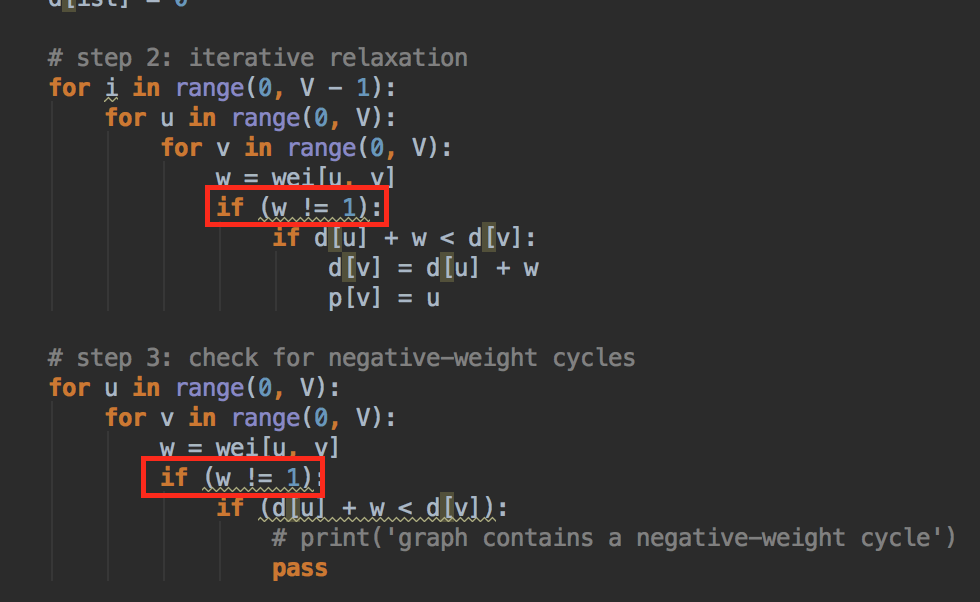
\includegraphics{changes}\label{changes}
\end{figure}

Otherwise, the code is the same as from tutorials, so I will not include it in full here.\\ \\
The following code calculates the longest path from $v_{s}$ to $v_{f}$.

\begin{python}
    adjusted_weights = -1 * weights
    longest_path = updated_bellman_ford(
        virtual_start, virtual_finish, adjusted_weights)[1:-1:2]
\end{python}
printing this longest path in Figure \ref{long} gives [0,1,4].
\begin{figure}[h]\label{long}
\caption{longest path from virtual start to virtual finish}
\centering
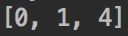
\includegraphics[scale=0.9]{long}
\end{figure}

\bcattention \quad since our adjacency matrix uses the ordering $0_{s} 1_{s} \dots 12_{s} 0_{f} 1_{f} \dots 12_{f} v_{s} v_{f}$, our output will follow the same style. Namely, $[v_{s},node1_{s},node1_{f},node2_{s},node2_{f},\dots,nodek_{s},nodek_{f},v_{f}]$. But the virtual nodes are just dummy nodes. We're really trying to find the longest dependent job sequence, and they ensure that we have. So we need to bring our results back to the normal scale, by removing the first and last values, then taking every second value. The python slice [1:-1:2] does exactly this. \\ \\

So $0 \to 1 \to 4$ is the longest string of jobs.

\section{Finding the earliest start and stop times}
In this section, we adopt the following notation. For a job $m \in \{0,1,\dots,12 \}$, we write $b_{m}$ for the path 
$$ b_{m} = m_{s} \to m_{f} $$

The first thing to realise is that the earliest start time for job $m \in \{ 0, \dots, 12 \}$ is determined precisely by the length of the longest job sequence to $m$. \\ \\
This is clear. If job m has no dependencies, it can start right away. \\ 
But if there are job sequences that finish on job $m$, we need to wait for all of these job sequences to finish, before we can execute job m. More formally, if $$ b_{m_{1}} \to b_{m_{2}} \to \dots \to b_{m_{l}} \to b_{m}$$
is the longest path in the graph ending on $b_{m}$ , then the earliest time job m can start is $\sum_{i=1}^{l}len(b_{m_{i}}) = \sum_{i=1}^{l} \ \text{duration of job $m_{i}$}$ \\ \\
\begin{claim}
Let the longest job sequence that finishes on job m be $b_{m_{1}} \to \dots \to b_{m_{l-1}} \to b_{m}$. Then $\forall i \in \{ 1,\dots,l-1\}$ $$\text{the longest job sequence that finishes on job $m_{i}$ is} \ b_{m_{1}} \to \dots \to b_{m_{i-1}} \to b_{m_{i}}$$
\end{claim}

\begin{claimproof}
Suppose not. Then there exists a longer sequence to job i: $b_{k_{1}} \to \dots \to b_{k_{p}} \to b_{m_{i}}$, say. But then, $b_{k_{1}} \to \dots \to b_{k_{p}} \to b_{m_{i}} \to b_{m_{i+1}} \dots \to b_{m_{l-1}} \to b_{m}$ is a longer path to job m than the one we assumed to be. This is a contradiction.
\end{claimproof}
\\
This argument about there not existing a longer sequence to job i (or $b_{i}$), is the key to this section. And it is why the introduction of the virtual start and finish nodes is so useful, as it means the longest path from virtual start to virtual finish trails through the graph to give you the longest job sequence. \\ 

Due to these results, after finding the longest job sequence in the graph [0,1,4], we can simply remove the edge from $4_{f} \to v_{f}$. Then if we find the longest job sequence in the graph again, there will be no route from $v_{s}$ to $v_{f}$ via job 4, and we will find the second longest job sequence in the graph. Continuing in this way, removing one node at a time we can find all of the necessary remaining (shorter) job sequences to recover the earliest start and stop times.

In fact, we can remove more connections than just each job in the job sequence to the virtual finish node. After we have found the longest job sequence finishing at job $e$, $b_{c} \to b_{d} \to b_{e}$, say. We can remove the connection between the last pair of jobs in this path, d and e. For if there were another job sequence which could utilise this edge, $b_{c} \to b_{d} \to b_{e}$ would not be the longest job sequence in the graph (currently). This reduction means that there is one less edge for the Bellman Ford algorithm to iterate through, and slightly eases the time complexity.

We now have all the information we need to find the earliest start times (the earliest stop time is then just the duration of a job + its earliest start time). The algorithm to do this is as follows:

\begin{enumerate}
\item Determine the longest path in the graph.
\item  By the arguments above, you have the start and stop times for every job in that path. for (node in longest path) \{ update the earliest start time for that node if you haven't already \}
\item for (node in longest path) \{ remove connection from node to virtual finish.
IF len(longest path) > 1: remove the edge between the last pair in the longest path.
\}
\item If there are still jobs whose start time you haven't determined, GOTO 1. Else, finish.
\end{enumerate}

\bcattention \quad It occurred to me that another possible optimisation in this algorithm would be to iterate backwards through the longest job sequence, as you could terminate this loop as soon as you have reached a job whose time you have already settled. But this would not improve the time complexity in this situation for a number of reasons: In order to attack the problem this way you need to calculate the sum of the longest job sequence, which is an order of n operation anyway. Sure, np.sum is fast but the job sequence is not a numpy array, and converting each sequence to an array would cost even more time. This approach may be more effective when job sequences and dependencies are very large and complicated, but in this situation the overhead is too much for it to be useful. \\

Here is the python implementation for this section.

\begin{python}
def iterative_bell(adjusted_weights,start_stop):
    """
    This function uses the Bellman Ford algorithm to iteratively find
    the remaining job sequences in the graph. It adjusts the start_stop
    array

    :param adjusted_weights: A, the negative adjacency matrix
    :param start_stop: the list of earliest start and stop times to be
    edited and updated
    :return: the longest paths used to find the start_stop times
    """

    # create the longest paths list
    longest_paths = []

    # create a copy of the weight matrix
    temp_weights = np.copy(adjusted_weights)

    # create a boolean array of False's. removed_nodes[m] = True if
    # job m has been removed (its value of earliest start and stop
    # has been calculated).
    removed_nodes = np.zeros(13, dtype=bool)

    # a counter so we know when to stop.
    counter = 0

    while counter < 13:  #

        # find the longest path in the graph from virtual start
        # to virtual finish
        job_sequence = updated_bellman_ford(virtual_start,
                                            virtual_finish,
                                            temp_weights)[1:-1:2]

        # remove the connections from those jobs to virtual finish
        temp_weights[np.array(job_sequence)+13,virtual_finish] = 1
        # if we have at least 2 elements, remove the last pair
        if len(job_sequence) > 1:
            temp_weights[job_sequence[-2] + 13,job_sequence[-1]] = 1

        # determine the times using the algorithm derived
        current_time = 0  

        # iterate through the jobs in the job sequence
        for job in job_sequence:  

            # only add to start_times if you haven't already
            if not removed_nodes[job]:  
                # set it to the current time. i.e the sum of jobs before it
                start_stop[job, 0] = current_time  
                start_stop[job, 1] = current_time + job_duration[job]
                # add 1 to the counter
                counter += 1  

            # update current_time
            current_time += job_duration[job]  

        # set all of the nodes in this job sequence to True
        removed_nodes[job_sequence] = True  
        # add this job sequence to the list of longest paths
        longest_paths.append(job_sequence)
        
    return longest_paths
\end{python}

We store the longest paths to help with the creation of the Gantt diagram later.

This is the code to run this function

\begin{python}
    start_stop = np.zeros((13, 2), dtype=int)

    longest_paths_list = iterative_bell(adjusted_weights,start_stop)

    full = np.column_stack((data,start_stop))
    \end{python}

See Figure 5.1 for the start\_stop array.

\begin{figure}[h]
\caption{earliest start and stop times for each job - row with index i corresponds to job i}
\centering
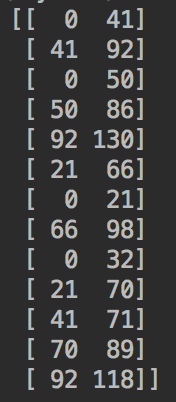
\includegraphics[scale=0.8]{lists}\label{startst}
\end{figure}

\section{Producing the Gantt chart}

Now we have our earliest start and stop times for each job, we can find one solution using a worker for each job, this finishes in the fastest time of 130 minutes. We are bound to 130 minutes because this is the earliest finishing time for job 4. See Figure \ref{first}.\\
We have optimised for time, but clearly not for workers. \\


\begin{figure}[h]
\caption{gantt chart using start and stop times}
\centering
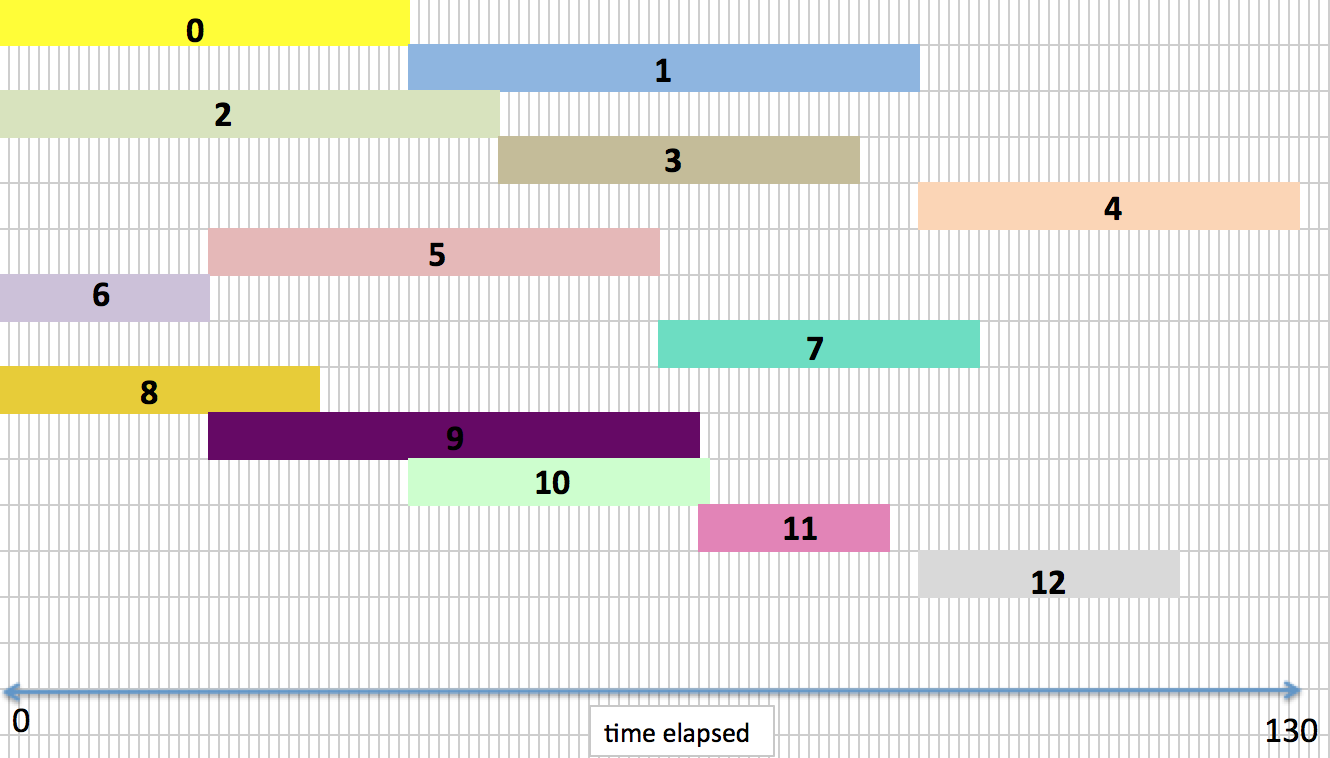
\includegraphics[scale=0.6]{initial}\label{first}
\end{figure}

At the end of section 1.4 we showed how the \textit{iterative\_bell} function found all of the longest job sequences in our graph. I print these in Figure \ref{second}

\begin{figure}[h]
\caption{The longest job sequences in the graph}
\centering
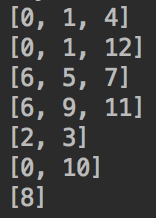
\includegraphics[scale=0.8]{longest}\label{second}
\end{figure}

Now, we can slide jobs up and down in the Gantt diagram as we please, without disturbing times or job dependencies. We should do so in accordance with the longest job sequences, in figure \ref{second} as we will inevitably waste less time between jobs. This sliding up and down results in the Gantt diagram in figure \ref{third}

\begin{figure}[h]
\caption{updated Gantt diagram}
\centering
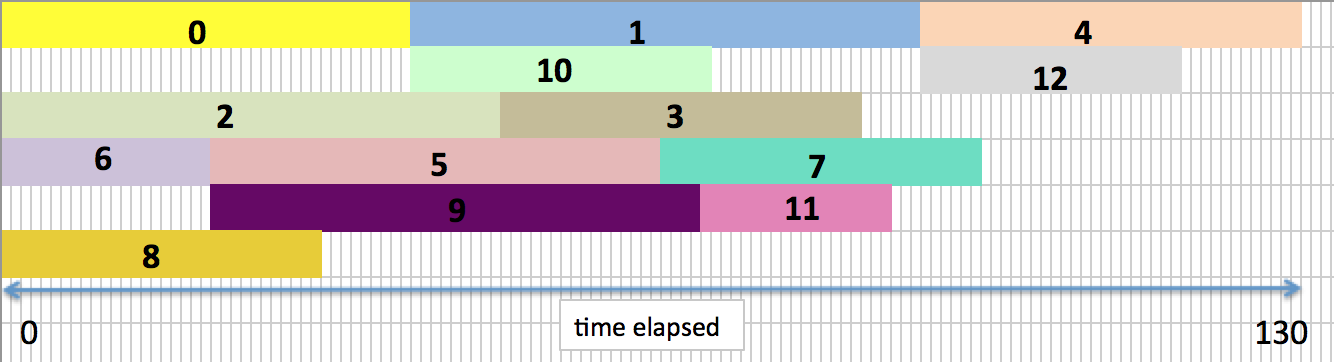
\includegraphics[scale=0.6]{group}\label{third}
\end{figure}

Some jobs are able to move freely as no jobs depend on them, and they depend on no others. Like job 8 for example. So we can move job 8 to the end of the $6 \to 5 \to 7$ row as its duration will still be less than 130. We then spot that we can move 12 to the end of the $9 \to 11$ row, and slot 10 between $2 \to 3$ while still respecting all job dependencies. This is shown in figure \ref{fourth}.

\begin{figure}[h]
\caption{Final Gantt diagram}
\centering
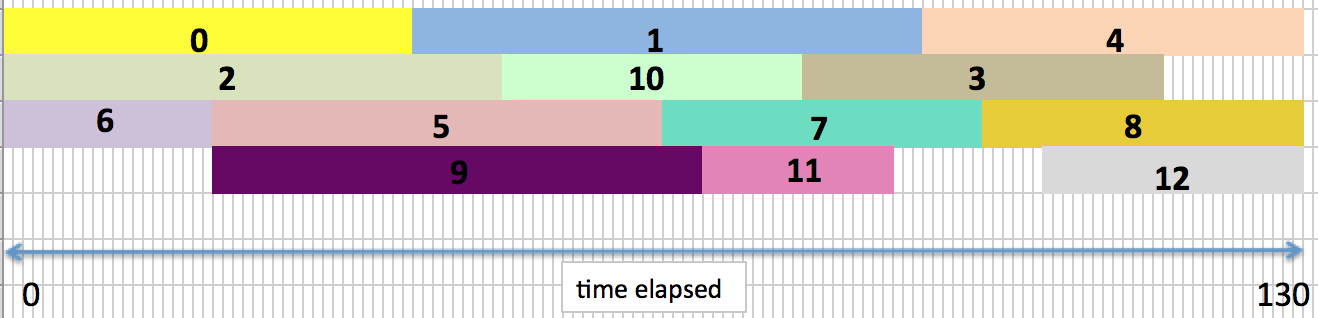
\includegraphics[scale=0.6]{final}\label{fourth}
\end{figure}

It is impossible to fit these jobs on three lines even if we ignore job dependencies, so we have optimised the workflow as required.
\end{document}


